\title{Pipeline Architecture}
\author{Brae Webb}
\date{\week{2}}

\maketitle

\section{Introduction}

Pipeline architectures take the attribute of modularity of a system to the extreme.
Pipeline architectures are composed of small well-designed components which can ideally be combined interchangeably.
In a pipeline architecture, input is passed through a sequence of components until the desired output is reached.
Almost every developer will have been exposed to software which implements this architecture.
Some notable examples are bash, hadoop, some older compilers, and most functional programming languages.

\begin{definition}[Pipeline Architecture]
    Components connected in such a way that the output of one component is the input of another.
\end{definition}


\begin{figure}[ht]
    \centering
\begin{tikzpicture}[>=latex']
    \tikzset{block/.style= {draw, rectangle, align=center,minimum width=2cm,minimum height=1cm},}

    \node [block] (input) {cat assignment.py};
    \node [block, right =2cm of input] (grep) {grep "f***"};
    \node [block, right =2cm of grep] (wc) {wc -l};
    \node [block, right =2cm of wc] (tee) {tee anger.txt};

    \path[draw,->]
                (input) edge (grep)
                (grep) edge (wc)
                (wc) edge (tee)
                ;
\end{tikzpicture}
\caption{An example of using bash's pipeline architecture to perform statistical analysis.}
\label{fig:bash-example}
\end{figure}

The de-facto example of a well-implemented pipeline architecture is bash,
we'll explore the philosophy that supports the architecture shortly.
The above diagram represents the bash command, \bash{cat assignment.py | grep "f***" | wc -l | tee anger.txt}.

\noindent
If you're unfamiliar with unix processes (start learning quick!),
\begin{description}
    \item[cat] Send the contents of a file to the output.
    \item[grep] Send all lines of the input matching a pattern to the output.
    \item[wc -l] Send the number of lines in the input to the output.
    \item[tee] Send the input to stdout and a file.
\end{description}

\section{Terminology}

As illustrated by Figure \ref{fig:pipe-filter}, a pipeline architecture consists of just two elements;

\begin{description}
    \item[Filters] modular software components, and
    \item[Pipes] the transmission of data between filters.   
\end{description}

\begin{figure}[ht]
    \centering
\begin{tikzpicture}[>=latex']
    \tikzset{block/.style= {draw, rectangle, align=center,minimum width=2cm,minimum height=1cm},}

    \node [block] (filter1) {Filter};
    \node [block, right =2cm of filter1] (filter2) {Filter};
    \node [block, right =2cm of filter2] (filter3) {Filter};

    \path[draw,->]
                (filter1) edge node[above] {Pipe} (filter2)
                (filter2) edge node[above] {Pipe} (filter3)
                ;
\end{tikzpicture}
\caption{A generic pipeline architecture.}
\label{fig:pipe-filter}
\end{figure}

\noindent Filters themselves are composed of four major types:

\begin{description}
    \item[Producers] Filters where data originates from are called producers, or source filters.
    \item[Transformers] Filters which manipulate input data and output to the outgoing pipe are called transformers.
    \item[Testers] Filters which apply selection to input data, allowing only a subset of input data to progress to the outgoing pipe are called testers.
    \item[Consumers] The final state of a pipeline architecture is a consumer filter, where data is eventually used.
\end{description}

The example in Figure \ref{fig:bash-example} shows how bash's pipeline architecture can be used to manipulate data in unix files.
Figure \ref{fig:bash-example-labelled} labels the bash command using the terminology of pipeline architectures.

\begin{figure}[H]
    \centering
\begin{tikzpicture}[>=latex']
    \tikzset{block/.style= {draw, rectangle, align=center,minimum width=2cm,minimum height=1cm},}

    \node [block,label=\color{gray}Producer] (input) {cat assignment.py};
    \node [block,label=\color{gray}Tester, right =2cm of input] (grep) {grep "f***"};
    \node [block,label=\color{gray}Transformer, right =2cm of grep] (wc) {wc -l};
    \node [block,label=\color{gray}Consumer, right =2cm of wc] (tee) {tee anger.txt};

    \path[draw,->]
                (input) edge (grep)
                (grep) edge (wc)
                (wc) edge (tee)
                ;
\end{tikzpicture}
\caption{Figure \ref{fig:bash-example} with labelled filter types.}
\label{fig:bash-example-labelled}
\end{figure}

\section{Pipeline Principles}
While the concept of a pipeline architecture is straightforward,
there are some principles which should be maintained to produce a well-designed and re-usable architecture.

\begin{definition}[One Direction Principle]
    Data should flow in one direction, this is the \textsl{downstream}.
\end{definition}

The data in a pipeline architecture should all flow in the same direction.
Pipelines should not have loops nor should filters pass data back to their \textsl{upstream} or input filter.
The data flow \textsl{is} allowed to split into multiple paths.
For example, Figure \ref{fig:analytics} demonstrates a potential architecture of a software which processes the stream of user activity on a website.
The pipeline is split into a pipeline which aggregates activity on the current page and a pipeline which records the activity of this specific user.

\begin{figure}
    \centering
    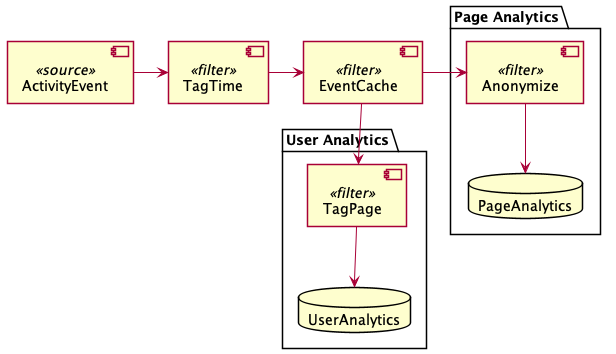
\includegraphics[width=0.8\textwidth]{diagrams/activity-tracking.png}
    \label{fig:analytics}
    \caption{Pipeline architecture for processing activity on a website for later analytics.}
\end{figure}

The One Direction Principle makes the pipeline architecture a poor choice for applications which require interactivity,
as the results aren't propagated back to the input source.
However, it is a good choice when you have data which needs processing with no need for interactive feedback.

\begin{definition}[Independent Filter Principle]\label{independent}
Filters should not rely on specific upstream or downstream components.
\end{definition}

In order to maintain the reusability offered by the pipeline architecture,
it is important to remove dependencies between individual filters.
Where possible, filters should be able to be moved freely.
In the example architecture in Figure \ref{fig:analytics},
the EventCache component should be able to work fine without
the TagTime component.
Likewise, EventCache should be able to process data if the
Anonymize filter is placed before it.

Producers and consumers may assume that they have no upstream or downstream filters respectively.
However, a producer should be indifferent to which downstream filter it feeds into.
Likewise a consumer should not depend on the upstream filter.

\begin{corollary}[Generic Interface]\label{interface}
The interface between filters should be generic.
\end{corollary}

Corollary \ref{interface} follows from Definition \ref{independent}.
In order to reduce the dependence on specific filters,
all filters of a system should implement a generic interface.
For example, in bash filters interface through the piping
of raw text data.
All unix processes should support raw text input and output.

\section{Conclusion}

A pipeline architecture is a good choice for data processing when interactivity is not a concern.
Conceptually pipelines are very simple.
Following the principles of a pipeline architecture will delivery a modular system which supports high reuse.
